\documentclass[t, screen, aspectratio=43]{beamer}
\usepackage[T1]{fontenc}
\usepackage[utf8]{inputenc}
\usepackage{epsf}
\usepackage{graphicx}
\usepackage{geometry}
\usepackage{tabularx}
\usepackage[table]{colortbl}
\usepackage{xcolor}
\usepackage{soul}
% Use the NTNU-temaet for beamer 
% \usetheme[style=ntnu|simple|vertical|horizontal, 
%     language=bm|nn|en, 
%     smalltitle, 
%     city=all|trondheim|alesund|gjovik]{ntnu2017}
\usetheme[style=helvet,language=en]{ntnu2017}

\usepackage[english]{babel}
\usepackage[style=numeric,backend=biber,natbib=false,sorting=none]{biblatex}

\title[Short title]{Ultra-Low Power PLL for Wake-up Receiver Applications}
\subtitle{Specialization Project Progress - 5th Week}
\author[C Nielsen]{Cole Nielsen}
\institute[NTNU]{Department of Electronic Systems, NTNU}
\date{27 September 2019 (Week 39)}
%\date{} % To have an empty date

\addbibresource{example.bib} % Add bibliography database

% Set the reference style to numeric.
% See here: http://tex.stackexchange.com/questions/68080/beamer-bibliography-icon
\setbeamertemplate{bibliography item}[text] 

% Set bibliography fonts to a small size.
\renewcommand*{\bibfont}{\footnotesize}

\begin{document}

\begin{frame}
	\titlepage%
\end{frame}

% Alternatively, special title page command to get a different background
% \ntnutitlepage

% #############################################################################
% Timeline
% #############################################################################
\begin{frame}
	\frametitle{Autumn Timeline}
	\begin{table}[htb!]
		\tiny
		\centering
		\vspace{-1em}
		\def\arraystretch{1.5}		
		\setlength\arrayrulewidth{0.75pt}
		\setlength{\tabcolsep}{1em} % for the horizontal padding
		\begin{tabular}{|l|l|l|l|}
			\hline 
			\rule[-1ex]{0pt}{2.5ex} \cellcolor{gray!40}\textbf{Week Number} & \cellcolor{gray!40}\textbf{Dates} &\cellcolor{gray!40}\textbf{Tasks} & \cellcolor{gray!40}\textbf{Outcomes}\\ 
			\hline 
			\rule[-1ex]{0pt}{2.5ex} \cellcolor{red!20}\textbf{36}& \cellcolor{red!20}2.9 - 8.9 & \cellcolor{red!20}Review PLL Design & \cellcolor{red!20}Refreshed Knowledge\\ 
			\hline 
			\rule[-1ex]{0pt}{2.5ex} \cellcolor{red!20}\textbf{37}& \cellcolor{red!20}9.9 - 15.9 & \cellcolor{red!20}Modeling/simulation (set up) & \cellcolor{red!20}--\\ 
			\hline 
			\rule[-1ex]{0pt}{2.5ex} \cellcolor{red!20}\textbf{38}& \cellcolor{red!20}16.9 - 22.9 & \cellcolor{red!20}Modeling/simulation &\cellcolor{red!20} TDC/DCO Requirements\\ 
			\hline 
			\rule[-1ex]{0pt}{2.5ex} \cellcolor{green!20}\textbf{39}& \cellcolor{green!20}23.9 - 29.9& \cellcolor{green!20}Modeling/simulation& \cellcolor{green!20}Loop Filter/Digital Algorithms\\ 
			\hline 
			\rule[-1ex]{0pt}{2.5ex} \cellcolor{blue!20}\textbf{40}& \cellcolor{blue!20}30.9 - 6.10& \cellcolor{blue!20}Modeling/simulation& \cellcolor{blue!20}\color{red}{\textbf{Loop filter,}} \color{black}{Ideal implementation in Cadence}\\ 
			\hline 
			\rule[-1ex]{0pt}{2.5ex} \textbf{41}& 7.10 - 13.10& Circuit Research & DCO/Divider topologies\\ 
			\hline 
			\rule[-1ex]{0pt}{2.5ex} \textbf{42}& 14.10 - 20.10& Circuit Research & TDC/other topologies\\ 
			\hline 
			\rule[-1ex]{0pt}{2.5ex} \textbf{43}& 21.10 - 27.10& Circuit Implementation& Digital logic (schematic)\\ 
			\hline 
			\rule[-1ex]{0pt}{2.5ex} \textbf{44}& 28.10 - 3.11& Circuit Implementation& DCO (schematic)\\ 
			\hline 
			\rule[-1ex]{0pt}{2.5ex} \textbf{45}& 4.11 - 10.11& Circuit Implementation& Divider/other (schematic)\\ 
			\hline 
			\rule[-1ex]{0pt}{2.5ex} \textbf{46}& 11.11 - 17.11& Circuit Implementation (TDC)& \\ 
			\hline 
			\rule[-1ex]{0pt}{2.5ex} \textbf{47}& 18.11 - 24.11& Circuit Implementation (TDC)& TDC (schematic)\\ 
			\hline 
			\rule[-1ex]{0pt}{2.5ex} \textbf{48}& 25.11 - 1.12& Full Circuit testing & Testbenches, find bugs, design fixes\\ 
			\hline 
			\rule[-1ex]{0pt}{2.5ex} \textbf{49}& 2.12 - 8.12& Full Circuit testing& Design Fixes/iteration\\ 
			\hline 
			\rule[-1ex]{0pt}{2.5ex} \textbf{50}& 9.12 - 15.12& --& --\\ 
			\hline 
		\end{tabular}
		\begin{flushleft}\textbf{Legend:} \colorbox{red!20}{\textbf{Done}} \colorbox{green!20}{\textbf{Current}}  \colorbox{blue!20}{\textbf{Revised}}
		% *I will write the report simultaneously with the work.
		\end{flushleft}
		% \caption{Assigned specifications for branch line hybrid design.}
		% \label{asgn_specs}
	\end{table}   
\end{frame}


% #############################################################################
% This week
% #############################################################################

\begin{frame}
	\frametitle{Timeline Tasks}
	\begin{block}{This week}
		\begin{itemize}
			\footnotesize
			\item \textbf{Primary:} Loop analysis, requirements definition
			\begin{itemize}
				\footnotesize
				\item Design open loop filter design to meet closed loop requirements.
				\begin{itemize}
					\item Dependent on DCO properties ($k_{DCO}$, $f_0$, tuning range).
					\item Difference equation implementing discrete time 2nd order IIR filter.
				\end{itemize} 
				\item Datapath requirements (fixed-point resolution)
			\end{itemize} 
		\end{itemize}    
	\end{block}
	\begin{block}{Next week - \color{red} \textbf{Revised}}
		\begin{itemize}
			\footnotesize
			\item \textbf{Primary:} Ideal component PLL implementation in Cadence, \color{red} continue loop filter work.
			\begin{itemize}
				\footnotesize
				\item Ideal component PLL implementation is not a lot of work.
				\item Loop filter very critical, spend more time on this.
				\begin{itemize}
					\footnotesize
					\item Need to make Verilog description of loop filter for simulation in Cadence.
				\end{itemize}
			\end{itemize} 
		\end{itemize}    
	\end{block}
\end{frame}

% #############################################################################
% sim/modeling approach
% #############################################################################

\begin{frame}
	\frametitle{Loop Filter}
	\begin{block}{Original Attempt}
		\vspace{-.2em}
		\vspace{-0.5em}
		\center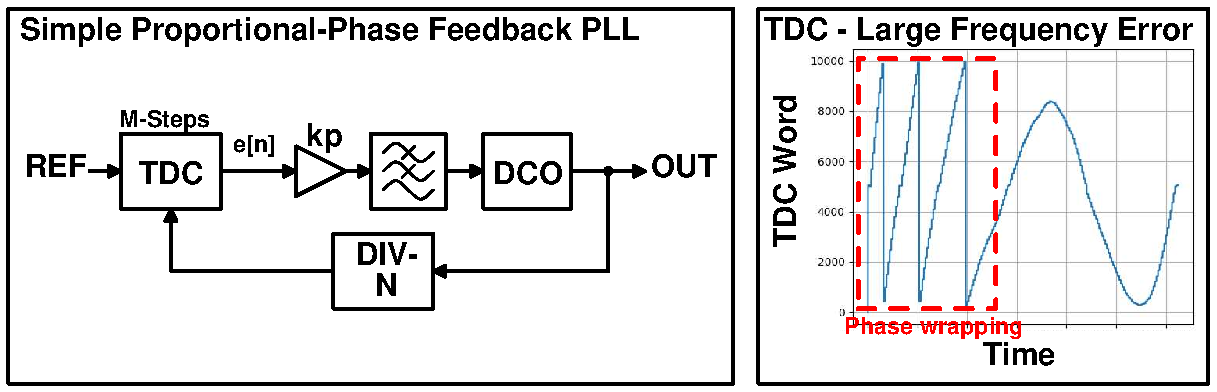
\includegraphics[width=0.75\textwidth, angle=0]{phase_wrap.pdf}
		\vspace{-0.5em}
		\begin{itemize}
			\footnotesize
			\item Started with simple PLL loop with proportional-phase fed into loop filter (LF).
			\begin{itemize}
				\scriptsize
				\item Not stable at large frequency offset, due to frequency wrapping. At the TDC:
				\tiny
				\begin{equation}
					\Delta \phi = \frac{2\pi \Delta f T}{N} \rightarrow T_{wrap} = \frac{N}{\Delta f}
				\end{equation}
				\scriptsize
				\item Upon cold start, $\Delta f$ is expected to be up to 100 MHz, N=150 $\rightarrow T_{wrap} = $ 1.5 $\mu$s
				\begin{itemize} 
					\scriptsize
					\item $f_{wrap} \sim$  600 kHz, this is unstable with a loop bandwidth of 100 kHz.
				\end{itemize}
				\item Must opt for alternate loop structure.
			\end{itemize}
		\end{itemize} 	
	\end{block}
\end{frame}


\begin{frame}
	\frametitle{Loop Filter}
	\begin{block}{New Approach}
		\vspace{-0.5em}
		\center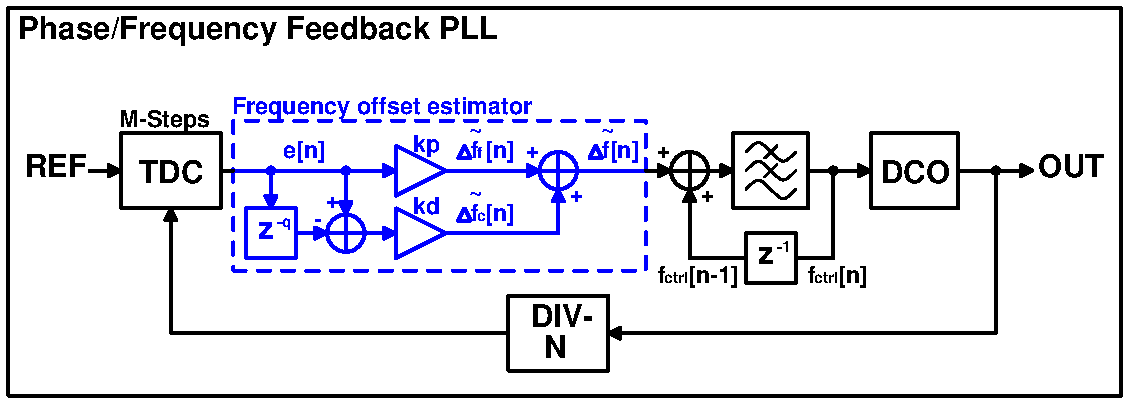
\includegraphics[width=0.75\textwidth, angle=0]{more_advanced.pdf}
		\vspace{-0.5em}
		\begin{itemize}
			\footnotesize
			\item Two-fold approach: utilize fine and coarse frequency offset estimation.
			\begin{itemize}
				\scriptsize
				\item Coarse frequency estimator to handle high frequency offset (e.g. cold start-up).	
				\item Fine frequency estimator for near steady state.
			\end{itemize}
			\item Offset estimates are summed with previous oscillator tuning word (OTW, also $f_{ctrl}$ here), then low passed filtered to yield new OTW. 
			\begin{itemize}
				\scriptsize
				\item Low pass filter loop keeps steady state.	
				\item Frequency estimator updates if any changes detected.
			\end{itemize}			
		\end{itemize} 	
	\end{block}
\end{frame}

\begin{frame}
	\frametitle{Loop Filter}
	\begin{block}{Coarse frequency offset estimation}
		\vspace{-0.5em}
		\center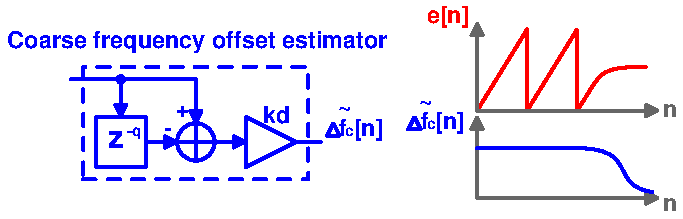
\includegraphics[width=0.5\textwidth, angle=0]{coarse_est.pdf}
		\begin{itemize}
			\footnotesize
			\item \textbf{Coarse frequency estimation:} Given M-step TDC, outputting phase error signal e$_\phi$[n], and a divider modulus N
			\tiny
			\vspace{-1em}
			\begin{equation}
				\Delta \phi_{DCO}[n; q] = N\cdot\Delta \phi_{REF}[n] = 2\pi \frac{N}{M}\left( e_\phi[n]-e_\phi[n-q]\right ),\hspace{2em} \Delta \phi_{DCO}[n; q] = \Delta \omega_{DCO}[n]qT_{ref} = 2\pi q \frac{\Delta f_{DCO}}{f_{ref}}
			\end{equation}
			\vspace{-1em}
			\begin{equation}
				\Delta f_{DCO} = \frac{f_{ref}}{q}\frac{N}{M}\left( e_\phi[n]-e_\phi[n-q]\right )
			\end{equation}				
			\footnotesize	
			\item Is a discrete differentiator, with gain coeficient to convert $d\phi/dt$ to frequency. 
			\begin{itemize}
				\scriptsize
				\item Rejects phase wrapping.	
				\item Useful in coarse frequency range calibration. Can detect fast if frequency offset too large.
				\item Delay q is used to increase frequency resolution. 
			\end{itemize}			
		\end{itemize} 	
	\end{block}
\end{frame}


\begin{frame}
	\frametitle{Loop Filter}
	\begin{block}{Coarse frequency offset estimation - continued}
		\begin{itemize}
			\footnotesize
			\item Given DCO gain $K_{DCO}$, the gain $K_d$ of the filter is:
			\tiny
			\vspace{-0.5em}
			\begin{equation}
				K_{d} = \frac{f_{ref}}{qK_{DCO}}\frac{N}{M}\left( e_\phi[n]-e_\phi[n-q]\right )
			\end{equation}				
			\footnotesize	
			\item Gate the coarse estimator off if $e_\phi[n]-e_\phi[n-q]$ < some threshold:
			\begin{itemize}
				\scriptsize
				\item Offset small enough, allow to run as classical phase-detector mode.
			\end{itemize}	
		\end{itemize} 
	\end{block}
	\begin{block}{Fine frequency offset estimation}
		\begin{itemize}
			\footnotesize
			\item Proportional signal of phase error to estimate frequency error.
			\item Used in near-steady state. Loop will regulate to keep phase locked.
			\item Classical PLL operating mode.
		\end{itemize} 	
	\end{block}
\end{frame}


\begin{frame}
	\frametitle{Loop Filter}
	\begin{block}{Modified implementation - PID}
		\vspace{-0.5em}
		\center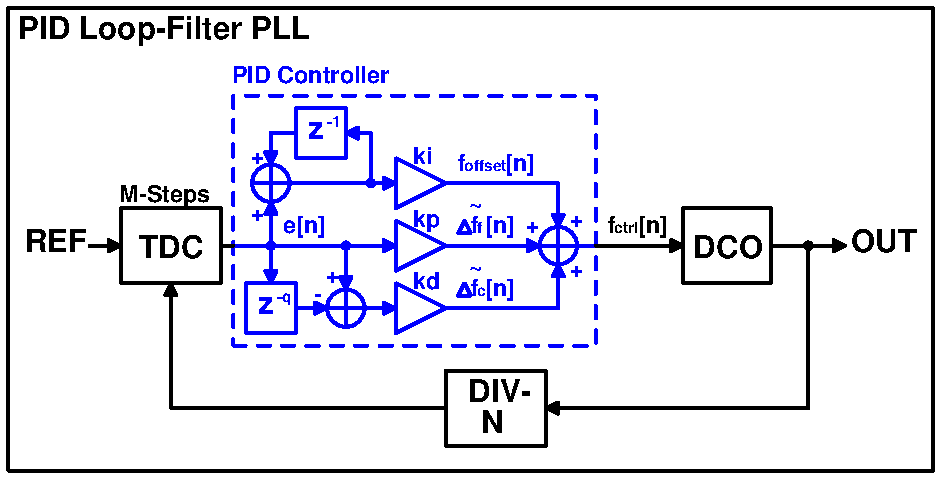
\includegraphics[width=0.5\textwidth, angle=0]{pid_pll.pdf}
		\vspace{-0.5em}
		\begin{itemize}
			\footnotesize
			\item On the observation that the loop filter was basically a PID controller.
			\begin{itemize}
				\scriptsize
				\item Add integral term to complete PID. Integral term keeps track of steady state offset of OTW, ideally yields 0 steady state error. 
				\item Derivative term \textit{only} used to perform coarse adjustment.
				\item Near/in steady, behaves as \textbf{PI controller}. 
			\end{itemize}
			\item 
		\end{itemize} 	 
	\end{block}
\end{frame}


\begin{frame}
	\frametitle{Loop Filter}
	\begin{block}{Loop Filter Gain Coefficients}
		\begin{itemize}
			\footnotesize
			\item On the observation that the loop filter was basically a PID controller.
			\begin{itemize}
				\scriptsize
				\item Add integral term to complete PID. Integral term keeps track of steady state offset of OTW, ideally yields 0 steady state error. 
				\item Derivative term used to perform coarse adjustment.
				\item Near/in steady, behaves as PI controller. 
			\end{itemize}
			\item 
		\end{itemize} 	 
	\end{block}
\end{frame}

% #############################################################################
% DCO
% #############################################################################

\begin{frame}
	\frametitle{DCO}
	\begin{block}{Performance criteria}
		\vspace{-.2em}
		\begin{itemize}
			\scriptsize
			\item Resolution set by frequency accuracy requirements, quantization noise.
			\item Quantization noise is manifested here as:
			\begin{itemize}
				\scriptsize			
				\item Reference spurs resulting from deterministic components of signal.
				\item A quasi-random noise signal when lock is achieved.
				\begin{itemize}
					\scriptsize			
					\item Results from stochastic toggling of $\sim$ 1 LSB of DCO tuning word to track low frequency variations.
					\item Rolloff of -20 dB/decade at low frequency (same as ring oscillator), -40 dB/decade at high frequencies.
				\end{itemize} 				
			\end{itemize} 
		\vspace{-1em}
		\center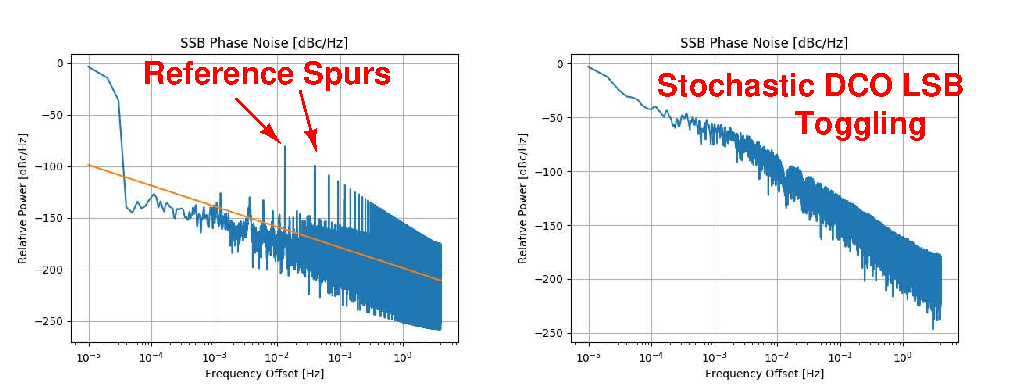
\includegraphics[width=0.7\textwidth, angle=0]{quant_noise.pdf}
		\vspace{-0.5em}  
		\end{itemize}    
	\end{block}
\end{frame}

\begin{frame}
	\frametitle{DCO}
	\begin{block}{Requirements based on reference spurs}
		\vspace{-.2em}
		\begin{itemize}
			\footnotesize
			\item Worst case reference spur level.
				\begin{itemize}
					\scriptsize			
					\item DCO tuning word toggling up/down 1 LSB every reference cycle.
				\end{itemize} 	
			\item With $f_0$ = 2.4 GHz, $f_{clk}$ = 16 MHz:
			\begin{itemize}
				\scriptsize			
				\item 52 kHz per LSB (i.e. $K_{DCO}$) is needed for a maximum -60 dBc reference spur level. 
			\end{itemize} 
		\end{itemize}  
		\vspace{-1em}
		\center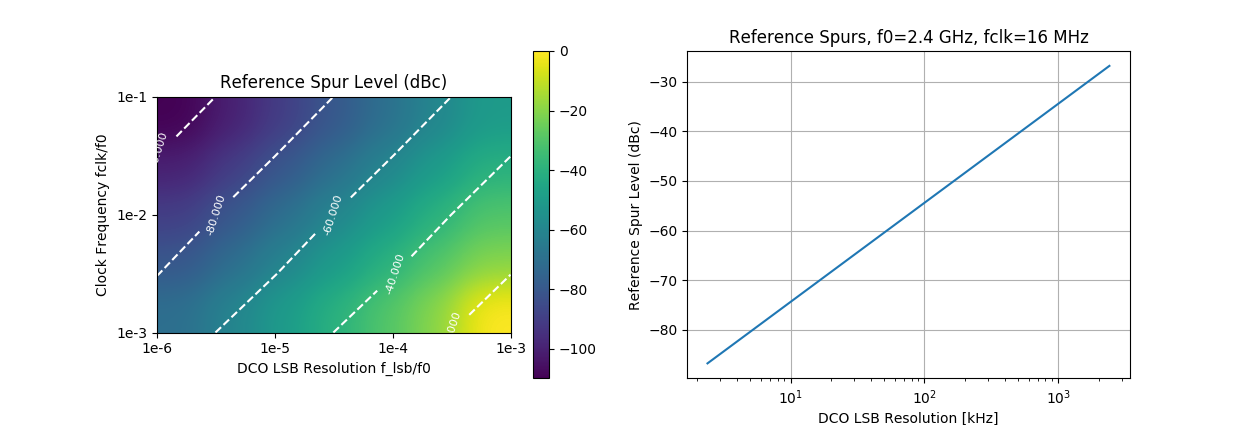
\includegraphics[width=1.0\textwidth, angle=0]{refspur_level.png}
		\vspace{-0.5em}  
	\end{block}
\end{frame}

\begin{frame}
	\frametitle{DCO}
	\begin{block}{Requirements from steady state tracking of stochastic variation.}
		% \vspace{-.2em}
		\begin{minipage}{7cm}
			\vspace{1em}
			\begin{itemize}
				\scriptsize
				\item In steady state, DCO tuning word will vary occassionaly by $\sim$ 1 LSB to track stochastic frequency changes.
				\begin{itemize}
					\tiny
					\item This generates noise and should be less than the thermal phase noise of DCO.		
					\item Very pessimistic estimate here (assumes abrupt frequency change). Abrupt frequency steps contribute 1/$\Delta f$ dependent component to phase noise.
				\end{itemize} 
				\item Theoretical ring oscillator phase noise limit from [2]:
				\tiny
				\begin{equation}
					PN_{min}(\Delta f)= 10\log 10\left(\frac{7.33k_BT}{P}\left(\frac{f_0}{\Delta f}\right)^2\right)
				\end{equation}
				\scriptsize
				\item If $f_0$ = 2.4 GHz, P = 50 $\mu$W, $\Delta f$= 1 MHz, T = 293K, $\rightarrow$ \textbf{PN < -84.7 dBc/Hz} from this noise process.
				\begin{itemize}
					\scriptsize			
					\item LSB resolution of \textbf{50 kHz} seems feasible. Will have to verify with full PLL sim to account for loop dynamics.
				\end{itemize} 
			\end{itemize}  
		\end{minipage}%
		% \hspace{-0.5cm}
		\begin{minipage}{5cm}
			% \vspace{-1.5em}
			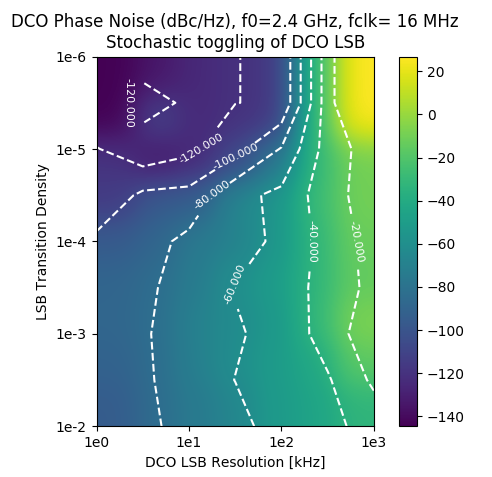
\includegraphics[width=1\textwidth, angle=0]{lsb_stochastic_pn.png}
			% \vspace{-0.5em}  
		\end{minipage}%
	\end{block}
\end{frame}

\begin{frame}
	\frametitle{DCO}
	\begin{block}{Accuracy and Linearity}
		\vspace{-.2em}
		\begin{itemize}
			\footnotesize
			\item Frequency accuracy.
				\begin{itemize}
					\scriptsize			
					\item Indeterminate IF assumed for wake up receivers, so accuracy not so critical.
					\item If RF bandwidth of receiver > PLL bandwidth, reasonable assumption is maximum frequency offset (accuracy) should be < PLL bandwidth.
					\item Current PLL bandwidth spec is 100 kHz, suggested 50 kHz LSB step from quantization noise analysis is sufficient?
					\begin{itemize}
						\scriptsize			
						\item This is assuming accuracy is tied to DCO resolution.
					\end{itemize} 
				\end{itemize} 	
			\item Linearity:
			\begin{itemize}
				\scriptsize			
				\item Integral non-linearity over the tuning DCO range is not important, so no spec for INL is suggested. Should be locally linear (constrains DNL).
				\item Monotonicity is essential, so must strictly have DNL < 1 LSB.
			\end{itemize} 
		\end{itemize}  
	\end{block}
\end{frame}

% #############################################################################
% TDC
% #############################################################################

\begin{frame}
	\frametitle{TDC}
	\begin{block}{Phase Noise Modeling}
 		\begin{itemize}
			\scriptsize
			\item Based on a phase-domain model for PLL phase noise from Michael Perrot [1].

		\end{itemize}  

		\begin{minipage}{5cm}
			\tiny
			\begin{equation}
				S_{\phi,out}(f)= f_{clk}\cdot\left| 2\pi NG(f) \right|^2\cdot\frac{\Delta t_{del}^2}{12}
			\end{equation}
			\begin{equation}
				G(f)= \frac{A(f)}{1 + A(f)}
			\end{equation}
		\end{minipage}
		\begin{minipage}{6cm}
			% \vspace{-1em}
			\center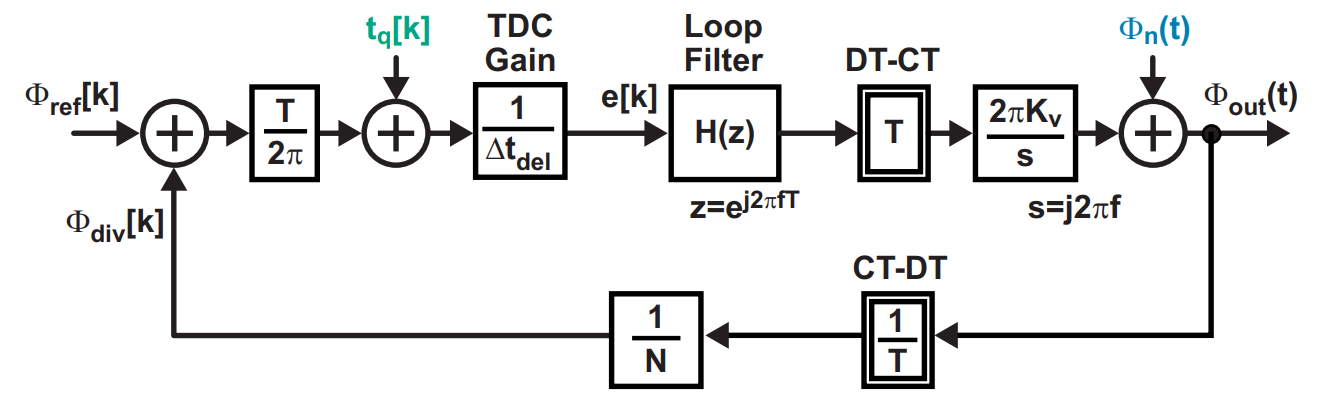
\includegraphics[width=1\textwidth, angle=0]{pll_loop.png}
			% \vspace{-0.5em}
		\end{minipage}
 		\begin{itemize}
			\scriptsize
			\item $S_{\phi,out}(f)$ is the TDC phase noise component, N is the divider modulus, G(f) is the closed loop PLL transfer function, A(f) is the open loop transfer function, $\Delta t_{del}$ is the TDC time resolution.
			\item G(0) = 1, and G(f) $\approx$ 1 for f $\in$ [0, $f_{CBW}$], where $f_{CBW}$ is the closed loop bandwidth.

		\end{itemize}  
	\end{block}
\end{frame}


\begin{frame}
	\frametitle{TDC}
	\begin{block}{Phase Noise Modeling}
		\begin{itemize}
			\footnotesize
			\item Naive estimate for TDC time resolution:
			\begin{itemize}
				\scriptsize
				\item Phase noise flat within closed-loop bandwidth. This component dominates power of the integrated phase noise a PLL with low TDC-resolution.
				\item Use Residual frequency modulation equation and equation 2 (TDC phase noise) to estimate $\Delta t_{del}$. Integrate in f $\in$ [0, $f_{CBW}$]
			\end{itemize} 
			\begin{equation}
				\Delta f_{RFM} = 2\int_{f_a}^{f_b}f^2*PN(f)df
			\end{equation}
			\item With $f_{clk}$ = 16 MHz, N = 150 (for 2.4 GHz synthesis), $\Delta f_{RFM}$ < 107 kHz to meet BER requirement, and $f_{CBW}$ = 100 kHz. (PLL presumed to have very low TDC resolution)
 			\begin{itemize}
				\scriptsize			
				\item $\Delta t_{del}$ < 3.8 ns
				\item Phase noise of TDC below $f_{CBW}$ is -47.7 dBc/Hz
				\item Equates to minimum of 16.4 quantization steps for TDC (4.03 bits).
				\item Assumptions of high phase noise and low resolution appear valid.

			\end{itemize} 
		\end{itemize}   
	\end{block}
\end{frame}

% #############################################################################
% Loop Dynamics (continuous)
% #############################################################################

% \begin{frame}
% 	\frametitle{Loop Dynamics}
% 	\begin{block}{Still To Do}
% 		\vspace{-.2em}
% 		\begin{itemize}
% 			\footnotesize
% 			\item Standard approach to used mixed continuous/discrete time mathematical model for DPLL. 
% 			\item Plot of RO phase noise (typical)
% 			\item Automatic analysis of performance (lock detection, residual phase modulation, lock-in/pull-in range).
% 			\item Automatic optimization (using gradient descent) of PLL parameters?
% 			\item Z-domain modeling of loop? Develop (by hand) some ideal transfer funtions for loop.

% 		\end{itemize}    
% 	\end{block}
% \end{frame}

% #############################################################################
% Specification
% #############################################################################

\begin{frame}
	\frametitle{Specification (unchanged)}
	\begin{block}{System Performance Targets}
		\scriptsize
		\begin{table}[h!]
			\centering
			\def\arraystretch{1.5}		
			\setlength\arrayrulewidth{0.75pt}
			\setlength{\tabcolsep}{1em} % for the horizontal padding
			\begin{tabular}{|l|r|l|l|}
				\hline 
				\rule[-1ex]{0pt}{2.5ex} \cellcolor{gray!40}\textbf{Parameter} & \cellcolor{gray!40}\textbf{Value} & \cellcolor{gray!40}\textbf{Unit }& \cellcolor{gray!40}\textbf{Notes}\\ 
				\hline 
				\rule[-1ex]{0pt}{2.5ex} \textbf{Frequency}  & 2.4-2.4835 & GHz & 2.4G ISM Band\\ 
				\hline 
				\rule[-1ex]{0pt}{2.5ex} \textbf{Ref. frequency} & 16 & MHz & Yields 6 channels \\ 
				\hline 
				\rule[-1ex]{0pt}{2.5ex} \textbf{Power} & $\leq$ 100  &$\mu$W & \\ 
				\hline 
				\rule[-1ex]{0pt}{2.5ex} \textbf{Residual FM} & $\leq$ 107  &kHz$_{RMS}$ & BER $\leq$ 1e-2, $f_{dev}$=$\pm$250 KHz\\ 
				\hline 
				\rule[-1ex]{0pt}{2.5ex} \textbf{Initial Lock Time} & $\leq$ 50 & $\mu$s & Upon cold start \\ 
				\hline 
				\rule[-1ex]{0pt}{2.5ex} \textbf{Re-lock Time} & $\leq$ 5 & $\mu$s & Coming out of standby \\ 
				\hline 
				\rule[-1ex]{0pt}{2.5ex} \textbf{Bandwidth} & 100 & kHz & (nominally), tunable \\ 
				\hline 
			\end{tabular} 
			% \caption{Assigned specifications for branch line hybrid design.}
			% \label{asgn_specs}
		\end{table}   
		Additionally: PLL output should support IQ sampling at LO frequency.
	\end{block}    
\end{frame}

\begin{frame}
	\frametitle{Specification (new)}
	\begin{block}{PLL Component Performance Targets}
		\scriptsize
		\begin{table}[h!]
			\centering
			\def\arraystretch{1.5}		
			\setlength\arrayrulewidth{0.75pt}
			\setlength{\tabcolsep}{1em} % for the horizontal padding
			\begin{tabular}{|l|r|l|l|}
				\hline 
				\rule[-1ex]{0pt}{2.5ex} \cellcolor{gray!40}\textbf{Parameter} & \cellcolor{gray!40}\textbf{Value} & \cellcolor{gray!40}\textbf{Unit }& \cellcolor{gray!40}\textbf{Notes}\\ 
				\hline 
				\rule[-1ex]{0pt}{2.5ex} \textbf{DCO LSB Resolution}  & $\leq$ 50  & kHz & Determined from quantization noise.\\ 
				\hline 
				\rule[-1ex]{0pt}{2.5ex} \textbf{DCO DNL} & < 1 & LSB & Ensures monotonicity \\ 
				\hline 
				\rule[-1ex]{0pt}{2.5ex} \textbf{TDC Resolution} & $\leq$ 3.8  & ns & \\ 
				\hline 
				\rule[-1ex]{0pt}{2.5ex} \textbf{TDC Resolution (bits)} & $\geq$ 4.03 &bits & \\ 
				\hline 
			\end{tabular} 
			% \caption{Assigned specifications for branch line hybrid design.}
			% \label{asgn_specs}
		\end{table}   
	\end{block}    
\end{frame}

% #############################################################################
% Architecture - block diagram
% #############################################################################

\begin{frame}
	\frametitle{Architecture (unchanged)}
	\begin{block}{Block Diagram}
	\center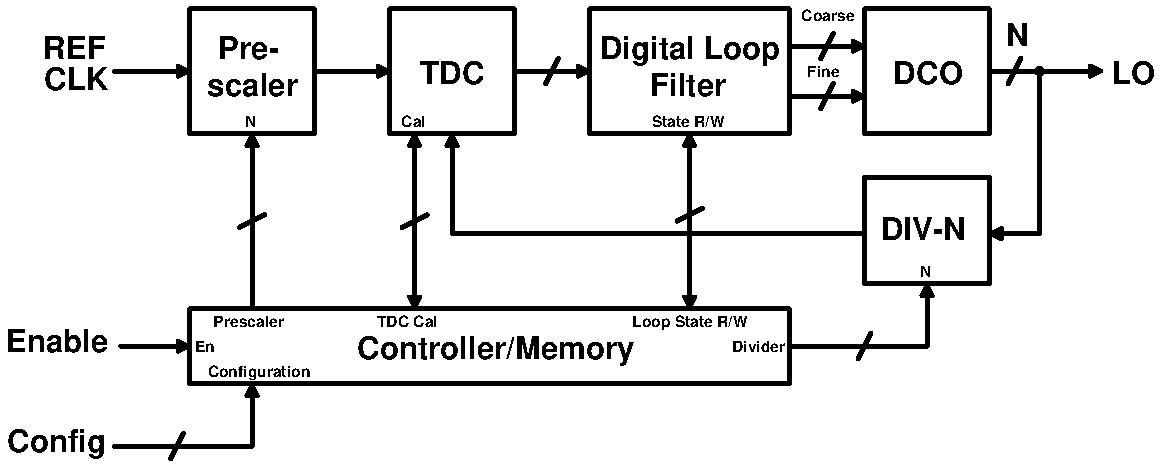
\includegraphics[width=0.75\textwidth, angle=0]{pll2.pdf}

	\end{block}
		\begin{block}{Power Targets}
		\vspace{-.1em}
		\begin{table}[htb!]
			\tiny
			\centering
			\def\arraystretch{1.5}		
			\setlength\arrayrulewidth{0.75pt}
			\setlength{\tabcolsep}{1em} % for the horizontal padding
			\begin{tabular}{|l|l|l|l|l|}
				\hline 
				\rule[-1ex]{0pt}{2.5ex} \cellcolor{gray!40}\textbf{DCO} & \cellcolor{gray!40}\textbf{TDC} & \cellcolor{gray!40}\textbf{Divider }& \cellcolor{gray!40}\textbf{Other} & \cellcolor{gray!40}\textbf{SUM} \\ 
				\hline 
				\rule[-1ex]{0pt}{2.5ex} 70 $\mu$W& 20 $\mu$W & 10 $\mu$W & $<<$ 1 $\mu$W & 100 $\mu$W\\ 
				\hline 
			\end{tabular} 
			% \caption{Assigned specifications for branch line hybrid design.}
			% \label{asgn_specs}
		\end{table}   
	\end{block}

\end{frame}


% #############################################################################
% project phases
% #############################################################################


\begin{frame}
	\frametitle{Project Phases}
	\begin{block}{Autumn 2019}
		\footnotesize
		\begin{itemize}
			\item System modeling and simulation.
			\begin{itemize}
				\footnotesize
				\item Learn PLL theory in detail
				\item Evaluate feasability of PLL architectures (counter, TDC-based)
				\item Determine requirements for TDC/DCO/Divider/logic (bits of resolution, accuracy etc) to meet PLL performance specifications.
				\item Determine digital logic for loop filter, validate stability and lock time performance.
			\end{itemize}
			\item Research ultra-low power circuit topologies to implement system components that will meet determined requirements.
			\item Translate component-level specifications into schematic-level circuit designs.
			\begin{itemize}
				\footnotesize
				\item Try, fail, try again until functional at schematic level.
				\begin{itemize}
					\footnotesize
					\item I expect the TDC to be difficult.
				\end{itemize}
			\end{itemize}      
		\end{itemize}
	\end{block}
\end{frame}

% #############################################################################
% Project phases slide 2
% #############################################################################


\begin{frame}
	\frametitle{Project Phases (continued)}
	\begin{block}{Spring 2020}
		\begin{itemize}
			\footnotesize
			\item Finalize schematic-level design.
			\item Estabilish thorough tests for PLL performance (automated?) to help in layout.
			\item Layout of PLL.
			\begin{itemize}
				\footnotesize
				\item Design iteration until design specs met.
				\item Probably very time consuming.
			\end{itemize}
			\item Full characterization/validation of design performance. 
			\begin{itemize}
				\footnotesize
				\item Comprehensive Corners/Monte-Carlo testing (time consuming??)
				\item More design iteration if new issues crop up...
			\end{itemize}
			\item Thesis paper writing.
		\end{itemize}
	\end{block}
\end{frame}

% #############################################################################
% References
% #############################################################################


\begin{frame}
	\frametitle{Project Phases (continued)}
	\begin{block}{Spring 2020}
		[1] "Digital Frequency Synthesizers", Michael Perrott, 2019.\\
		\hspace{16pt}\url{http://www.cppsim.com/PLL_Lectures/day4_am.pdf}\\
		\vspace{1em}
		[2] "Minimum Achievable Phase Noise of RC Oscillators",
	Navid et al. 2005
	\end{block}
\end{frame}


\end{document}
